% ----------------------------------------------------------
% Teste test3_1_e25b32class10_20231211_231229
% ----------------------------------------------------------
\subsubsection{Teste test3_1_e25b32class10_20231211_231229 - AlexNet (Is That a Santa)}

Informações utilizadas para o treinamento.

\begin{table}[ht]
   \centering
   \caption{Treinamento}
   \label{tab:modelos}
   \begin{tabular}{| c | c | }
      \hline 
      \textbf{Informação} & \textbf{Descrição} \\
      \hline \hline 
      Rede & AlexNet \\
      \hline
      Número de épocas & 25\\
      \hline
      Tamanho do lote & 32\\
      \hline
      Taxa inicial & 0.012 \\
      \hline
      Taxa de decaimento & 0.0006 \\
      \hline
      Total de classes & 10\\
      \hline
      Dataset & CIFAR-10\\
      \hline
   \end{tabular} 
\end{table}

Resultados obtidos após treinamento.

\begin{tabular}{lrrrr}
\toprule
  Unnamed: 0 &  precision &  recall &  f1-score &    support \\
\midrule
    airplane &   0.816888 &  0.8610 &  0.838364 &  1000.0000 \\
  automobile &   0.898622 &  0.9130 &  0.905754 &  1000.0000 \\
        bird &   0.790123 &  0.7040 &  0.744580 &  1000.0000 \\
         cat &   0.602444 &  0.6410 &  0.621124 &  1000.0000 \\
        deer &   0.818182 &  0.7560 &  0.785863 &  1000.0000 \\
         dog &   0.664655 &  0.7710 &  0.713889 &  1000.0000 \\
        frog &   0.878625 &  0.8180 &  0.847229 &  1000.0000 \\
       horse &   0.866667 &  0.8450 &  0.855696 &  1000.0000 \\
        ship &   0.901364 &  0.8590 &  0.879672 &  1000.0000 \\
       truck &   0.860465 &  0.8880 &  0.874016 &  1000.0000 \\
    accuracy &   0.805600 &  0.8056 &  0.805600 &     0.8056 \\
   macro avg &   0.809804 &  0.8056 &  0.806619 & 10000.0000 \\
weighted avg &   0.809804 &  0.8056 &  0.806619 & 10000.0000 \\
\bottomrule
\end{tabular}


\begin{figure}[ht]
 \begin{center}
   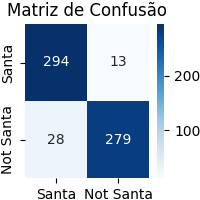
\includegraphics[scale=1]{tests/test3_1_e25b32class10_20231211_231229/confusion_matrix.png}
  \caption{Matriz de Confusão}
  \label{fig:fig03}
 \end{center}
\end{figure}

\begin{figure}[ht]
 \begin{center}
   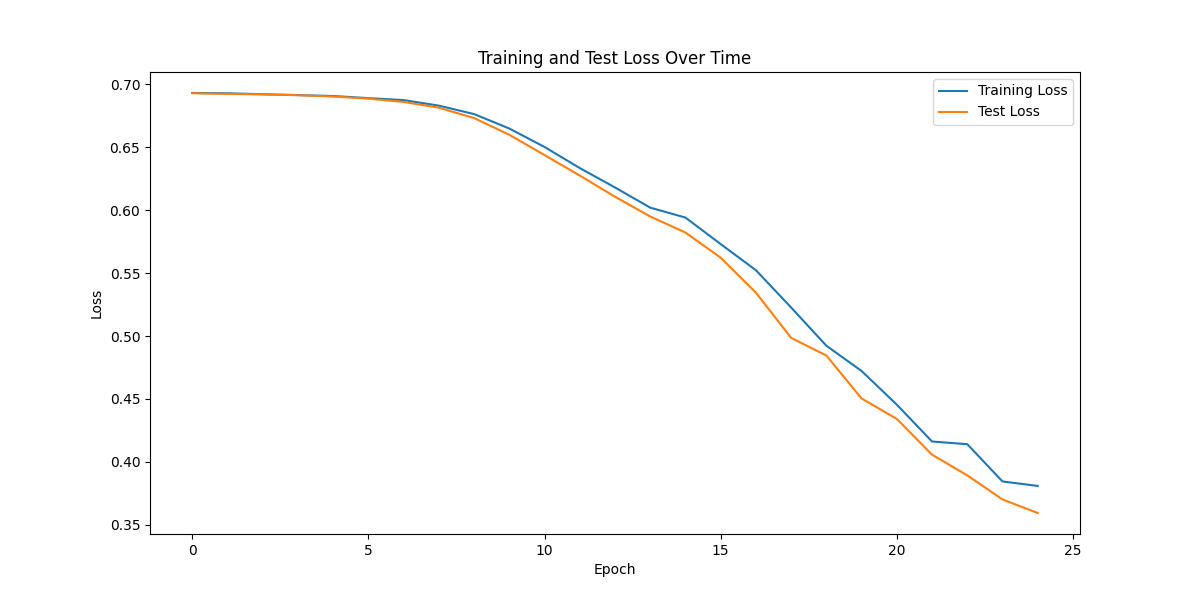
\includegraphics[scale=0.8]{tests/test3_1_e25b32class10_20231211_231229/loss_over_time.png}
  \caption{Gráfico de Perda}
  \label{fig:fig04}
 \end{center}
\end{figure}
